\documentclass[conference]{IEEEtran}

\IEEEoverridecommandlockouts

\usepackage{cite}
\usepackage{amsmath,amssymb,amsfonts}
\usepackage{algorithm}
\usepackage{algorithmic}
\usepackage{graphicx}
\usepackage{textcomp}
\usepackage{xcolor}
\usepackage{tikz}
\usepackage{adjustbox}
\usepackage[hyphens]{url}
\usepackage{booktabs}
\usepackage{array}
\usepackage{threeparttable}
\usepackage{enumitem}
\usetikzlibrary{arrows.meta,positioning,fit,calc,shapes.geometric}

\definecolor{lumoCyan}{RGB}{40,120,150}
\definecolor{lumoGreen}{RGB}{60,135,80}
\definecolor{lumoAmber}{RGB}{180,130,45}
\definecolor{lumoRose}{RGB}{175,80,85}
\definecolor{lumoGray}{RGB}{80,86,96}

\newcolumntype{L}[1]{>{\raggedright\arraybackslash}p{#1}}
\newcolumntype{C}[1]{>{\centering\arraybackslash}p{#1}}
\newcommand{\sys}{GDN Tree-Scan}
\newcommand{\code}[1]{\texttt{#1}}
\newcommand{\rowsep}{\specialrule{0.15pt}{1.2pt}{1.2pt}}

\begin{document}

\title{Served-Realization Tree Verification for Recurrent Hybrid Language Models}

\author{
    \IEEEauthorblockN{Zhiyuan Ma}
}

\maketitle

\begin{abstract}
\sys{} is a served-realization verifier for recurrent-hybrid speculative decoding in vLLM. It combines a forked FlashAttention-2 decode path with tree ancestry bias, a branch-local Triton Gated-DeltaNet scan/replay kernel, device-side multidraft commitment, and accepted-chain-only state publication for Qwen/Qwen3.6-27B-FP8. Unlike cache/scheduler-layer hybrid serving, algebraic state-sharing designs, or FPGA-oriented SSM speculation, the contribution is a fused vLLM/FA2/GDN realization at the target-verifier boundary. In a clean B=1, temperature-0.6, four-task SWE/Codex gate, the six-node root-branch tree reaches 23.88 token-weighted decode tokens/s versus 18.80 for native E5, a 27.0\% decode-throughput gain. The same run is only 4.0\% faster under a per-request-equal latency view, and end-to-end task wall time remains prefill-heavy. The empirical equivalence claim is scoped: the current gate is a sampled clear-margin p-rescore that closes within the observed native recurrent-oracle flip floor, not a full distribution-distance or request-cluster-bootstrap proof. We report the verifier contract, implementation seams, evidence gates, and failed routes that define this scoped decode-throughput result.
\end{abstract}

\begin{IEEEkeywords}
speculative decoding, recurrent models, Gated DeltaNet, vLLM, FlashAttention, ML systems
\end{IEEEkeywords}

\section{Introduction}

Speculative decoding accelerates autoregressive generation by drafting candidate tokens and asking the target model to verify them in parallel. Tree-shaped speculative decoding generalizes a single draft chain into a candidate token tree, improving the opportunity set for each target forward pass while preserving the target distribution under the verifier acceptance rule \cite{miao2023specinfer,chen2024sequoia,li2024eagle,wang2024opt}. For attention-only Transformer stacks, the central verifier problem is largely an ancestry problem: row \(i\) may attend to the prompt and its ancestors, but not to sibling branches \cite{miao2023specinfer,li2024eagle}.

Recurrent hybrid models break that simplification. Qwen 3.6-style hybrid stacks contain many Gated-DeltaNet (GDN) recurrent layers in addition to softmax-attention layers, so a valid tree row needs two path-local facts: attention ancestry and recurrent state lineage \cite{yang2024gated,qwen2026qwen36fp8}. We use recurrent for any layer whose next-token output depends on a carried serving state; GDN is linear attention with such a carried state. The verifier must ensure that a node's GDN state equals the state native sequential decode would have produced along that node's root-to-node path. If sibling rows share a packed recurrent accumulator, a correct attention mask can still verify tokens from an impossible recurrent history.

This paper reports a served verifier for a recurrent hybrid target inside vLLM. The contribution is not ``tree speculative decoding'' in the abstract. It is served-realization equivalence as an implementation target: forked FlashAttention-2 (FA2) tree bias for attention, branch-local GDN scan and accepted-chain replay for recurrence, and vLLM state publication that makes rejected branch state non-durable \cite{dao2023flashattention,kwon2023efficient,lumo2026artifact}. To our knowledge, this is the first served, fused vLLM+FA2+GDN tree verifier for a production hybrid target; it does not claim first hybrid speculation or first stateful tree decoding.

The measured result is deliberately narrow. We use E5 for the native five-step MTP spine and catN for N-node tree variants. In a clean B=1, temperature-0.6 deployment trace over four SWE/Codex tasks, cat6root, a six-node tree with a depth-5 native spine plus one root sibling, reaches 23.88 token-weighted decode tokens/s versus 18.80 for native E5, a 27.0\% decode-throughput gain. The root sibling is a depth-0 alternative: when native MTP would lose an event because the first spine token is rejected, the verifier can still commit the sibling branch, raising committed tokens/event from 4.11 to 4.82 while adding almost no verify-forward time. The per-request-equal latency view is 18.51 versus 17.80 tokens/s, or +4.0\%; this is useful but underweights long decode turns where most generated tokens occur. Both cat6root and cat9 close within the observed native recurrent-oracle flip floor in a 40-turn B=1 p-rescore, but full distribution-distance evidence, request-level bootstrap, more seeds, B=4, and Stage D timing remain open gates.

The paper makes three concrete contributions:
\begin{itemize}[leftmargin=*,noitemsep]
    \item A served verifier contract for recurrent hybrid token trees: attention ancestry, path-local GDN state, SpecInfer-style residual commitment, and accepted-chain-only durable publication.
    \item A vLLM/FA2/GDN implementation path that preserves native serving machinery where possible and adds tree-specific state only at explicit seams.
    \item An evidence ledger that separates clean B=1 decode throughput, per-request latency, recurrent-oracle p-rescore, end-to-end wall caveats, and contaminated or still-open measurements.
\end{itemize}

\section{Background and Related Work}

Speculative decoding uses a cheaper draft path to propose future tokens and verifies them with the target model. SpecInfer introduced tree-based speculative inference and parallel verification for LLM serving, while Sequoia, EAGLE-2, and OPT-Tree study hardware-aware, dynamic, or adaptive draft-tree structure \cite{miao2023specinfer,chen2024sequoia,li2024eagle,wang2024opt}. These systems establish the candidate-tree and verifier-acceptance framing, but the usual target-forward assumption is too high-level for a served recurrent hybrid.

STree is the closest prior work for stateful tree decoding. It extends tree speculative decoding to SSM and hybrid architectures by exploiting accumulated state-transition structure \cite{wu2025stree}. That framing transfers directly: stateful models need tree-aware state construction, not only tree-aware attention. The missing layer for this artifact is realization. The served target path has fp8/bf16 seams, branch co-residency, a specific FA2 attention implementation, GDN state writeback, and rejection sampling inside vLLM.

Recent hybrid serving and SSM speculation work sharpens the same boundary. SpecMamba identifies hidden-state backtracking, tree-verification incompatibility, and draft/target workload mismatch for Mamba speculative decoding, then targets an FPGA dataflow \cite{zhong2025specmamba}. Component-aware self-speculation shows that hybrid component structure matters: Falcon-H1 and Qwen3.5 behave differently because of how SSM/linear-attention components are integrated \cite{borobia2026component}. These papers explain why hybrid models create new verifier questions, but they do not close the vLLM/FA2/GDN served-realization path.

SGLang is the closest adjacent production comparison and should be treated carefully. Its hybrid-model writeup separates KV cache from request-level Mamba state, introduces MambaRadixCache, and handles speculative verification with independent state slots and parent tracing \cite{pytorch2025sglang}. Its Qwen3-Next documentation and speculative-decoding documentation show active support for GDN/MTP-style hybrid models \cite{sglang2026qwen,sglang2026specdocs}. That is not an apple-to-apple fused-kernel baseline for this paper: much of the mechanism is cache/scheduler-layer work, while this artifact's shipped contribution is lower in the stack, at the vLLM, forked-FA2, branch-local GDN scan/replay, and publication boundary \cite{sglang2026issue25587,lumo2026artifact}.

\begin{table*}[t]
\caption{Comparison layer for prior and adjacent work. The goal is to avoid promoting adjacent serving work into a direct fused-kernel baseline.}
\label{tab:prior}
\centering
\scriptsize
\begin{adjustbox}{width=\textwidth}
\begin{tabular}{L{0.18\textwidth} L{0.24\textwidth} L{0.26\textwidth} L{0.20\textwidth}}
\toprule
Line of work & What transfers & What breaks for this target & What \sys{} adds \\
\midrule
SpecInfer, Sequoia, EAGLE-2, OPT-Tree & Candidate trees, verifier acceptance, dynamic or hardware-aware shape selection \cite{miao2023specinfer,chen2024sequoia,li2024eagle,wang2024opt}. & The target verification forward is assumed to realize the target distribution once attention ancestry is correct. & Recurrent-state verification and deployment equivalence gates. \\
\rowsep
STree & Stateful models need tree-aware state construction \cite{wu2025stree}. & Algebraic state sharing is not the same as matching native served GDN under bf16/fp8 and vLLM writeback. & A GDN scan/replay kernel gated against native/deployment oracles. \\
\rowsep
SpecMamba & Hidden-state backtracking and tree verification are first-class SSM obstacles \cite{zhong2025specmamba}. & FPGA dataflow and FIFO verification are not a served GPU/vLLM path for Qwen GDN. & Fused GPU kernels, FA2/vLLM compatibility, and deployment gates. \\
\rowsep
Component-aware self-speculation & Hybrid component structure determines speculative viability \cite{borobia2026component}. & Research Python implementation leaves fused CUDA, batched verification, and cache sharing as systems gaps. & A fused served path for Qwen GDN tree verification. \\
\rowsep
SGLang hybrid serving & Adjacent production mechanisms: dual memory pools, MambaRadixCache, parent tracing, MTP/EAGLE surfaces \cite{pytorch2025sglang,sglang2026qwen,sglang2026specdocs}. & Cache/scheduler-layer mechanisms are not directly comparable to this fused vLLM GDN tree-scan kernel. & A different layer of realization: vLLM + forked FA2 tree bias + branch-local GDN scan/replay + observed recurrent-oracle gates. \\
\bottomrule
\end{tabular}
\end{adjustbox}
\end{table*}

\section{Claim Scope and Evidence Map}

The contribution is easiest to evaluate when each claim names its mechanism, measurement basis, and caveat. Table~\ref{tab:claims} makes that boundary explicit. The artifact receipts remain in the source trail; the paper body carries the facts needed to evaluate the argument without following every repository link.

\begin{table*}[t]
\caption{Claim, gate, and caveat map. The repository has a longer receipt ledger; this table keeps the academic claim boundary explicit.}
\label{tab:claims}
\centering
\scriptsize
\begin{adjustbox}{width=\textwidth}
\begin{tabular}{L{0.24\textwidth} L{0.26\textwidth} L{0.25\textwidth} L{0.17\textwidth}}
\toprule
Claim & In-paper evidence & Gate & Status and limit \\
\midrule
The systems contribution is served-realization equivalence for Qwen GDN in vLLM. & FA2 tree-bias decode, branch-local GDN scan/replay, device multidraft commitment, and accepted-chain-only durable publication. & All target-verifier surfaces consume the same tree descriptor and accepted path. & Closed for the shipped B=1 path; not a claim of first GDN speculation. \\
\rowsep
cat6root is faster than native E5 on clean B=1 decode throughput. & Table~\ref{tab:results}: 23.88 versus 18.80 token-weighted decode tokens/s. & Matched pure-decode GPU timer, probes off, temp-0.6, four SWE/Codex tasks. & +27.0\% decode-only; per-request-equal latency is +4.0\%. \\
\rowsep
cat9 and cat6root close within the native recurrent-oracle floor. & Section~\ref{sec:lossless}: 13.28\% and 13.09\% clear-margin flips versus native E5 at 12.90\%. & Each arm is compared with its own no-spec recurrent oracle in the B=1 p-rescore. & Closed for this 40-turn sample; no TV-distance or request-cluster bootstrap yet. \\
\rowsep
The measurement discipline is part of the result. & Speed runs disable probes; equivalence runs enable oracle capture; token-weighted and per-request views are reported separately. & No mixing of raw prompt probes, oracle capture, B=4 co-residency, or denominator conventions. & Prevents false speed wins and false equivalence failures; B=4 remains open. \\
\bottomrule
\end{tabular}
\end{adjustbox}
\end{table*}

\section{Verifier Contract}

\sys{} verifies an arbitrary candidate tree, not only the native MTP drafter used in the current implementation. The input contract is a prefix state, a parent array, candidate token ids, and sampling state. The output contract is stronger: after verification and commitment, the next served decode event must start from the same observable token prefix and recurrent state that native sequential decode would have reached on the accepted tokens, up to the observed native recurrent-oracle numerical floor.

\begin{table}[t]
\caption{Engineering form of the accepted-state verifier contract.}
\label{tab:contract}
\centering
\scriptsize
\begin{adjustbox}{width=\columnwidth}
\begin{tabular}{L{0.21\columnwidth} L{0.37\columnwidth} L{0.32\columnwidth}}
\toprule
Part & Formal content & Served implementation \\
\midrule
Inputs & Prefix state, parent array, candidate ids, sampling state. & vLLM tree packing plus multidraft metadata. \\
\rowsep
Attention & Row \(i\) sees prompt tokens and ancestors of \(i\), not siblings. & Forked FA2 adds \code{tree\_bias} before softmax; prefill stays native. \\
\rowsep
GDN & \(S_i=\mathrm{GDNStep}(S_{\mathrm{parent}(i)},x_i)\). & Triton GDN tree scan with branch-local \code{h\_cache}. \\
\rowsep
Acceptance & Apply the same residual speculative rule as target verification. & Device multidraft commit at temperature 0.6. \\
\rowsep
Publication & Only accepted-prefix tokens and their state become durable. & Accepted-chain replay and vLLM state writeback/remap. \\
\bottomrule
\end{tabular}
\end{adjustbox}
\end{table}

The contract can be summarized as an engineering invariant. Assume the tree contains only candidate ids and parent links; attention rows see only prefix plus ancestors; every GDN row is computed from its parent row's recurrent state; the committer applies the same residual rule as the target verifier; and durable state is replayed or published only for the accepted chain. Then the next served decode event has the same intended token-prefix and recurrent-state boundary as native sequential decode on the accepted prefix. The current evidence checks this boundary through recurrent-oracle p-rescore and targeted scan/replay gates rather than through a full distribution-distance proof \cite{miao2023specinfer}.

\begin{algorithm}[t]
\caption{Tree verification on a recurrent hybrid target}
\label{alg:tree}
\begin{algorithmic}[1]
\REQUIRE prefix state \(S_0\), candidate tree \(T=(V,E)\), token ids \(x_i\), sampling state
\STATE Pack candidate ids, parent indices, and ancestry masks into vLLM decode metadata.
\STATE Run softmax-attention layers with FA2 tree bias so row \(i\) sees prefix and ancestors only.
\FOR{each GDN layer}
    \FOR{each node \(i\) in topological order}
        \STATE Load \(S_{\mathrm{parent}(i)}\) from \(S_0\) or branch-local \code{h\_cache}.
        \STATE Compute \(S_i, o_i \leftarrow \mathrm{GDNStep}(S_{\mathrm{parent}(i)},x_i)\).
        \STATE Store \(S_i\) in \code{h\_cache[i]} for children.
    \ENDFOR
\ENDFOR
\STATE Apply the residual speculative acceptance rule on device.
\STATE Replay accepted path in native order and publish only accepted GDN/conv state.
\RETURN committed tokens and durable recurrent state for the next decode event.
\end{algorithmic}
\end{algorithm}

\section{System Design}

Figure~\ref{fig:pipeline} shows the served path. The drafter currently uses Qwen's native MTP head: root and spine tokens come from the same logits tensor, with runner-up leaves read as top-\(k\) candidates. The verifier should not depend on that drafter. Its stable boundary is a tree descriptor with parent indices, candidate ids, visibility masks, and accepted-path rows that can be replayed into native state.

\begin{figure}[t]
\centering
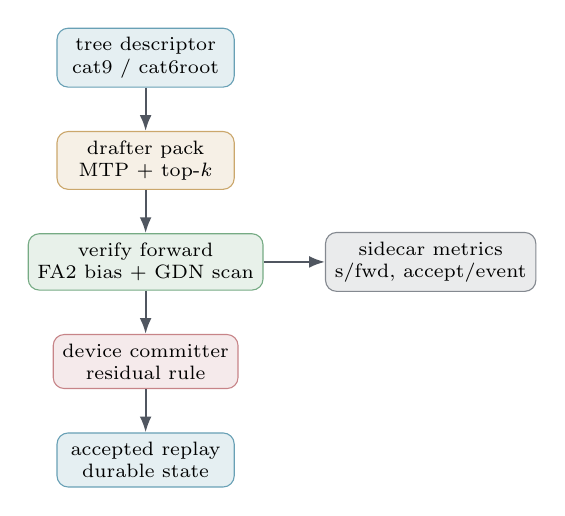
\begin{tikzpicture}[
    node distance=0.55cm,
    box/.style={rectangle, rounded corners, draw=#1!70, fill=#1!12, minimum width=2.25cm, minimum height=0.58cm, align=center, font=\scriptsize},
    arrow/.style={-{Latex[length=2mm]}, thick, draw=lumoGray}
]
\node[box=lumoCyan] (shape) {tree descriptor\\cat9 / cat6root};
\node[box=lumoAmber, below=of shape] (pack) {drafter pack\\MTP + top-\(k\)};
\node[box=lumoGreen, below=of pack] (verify) {verify forward\\FA2 bias + GDN scan};
\node[box=lumoRose, below=of verify] (commit) {device committer\\residual rule};
\node[box=lumoCyan, below=of commit] (publish) {accepted replay\\durable state};
\draw[arrow] (shape) -- (pack);
\draw[arrow] (pack) -- (verify);
\draw[arrow] (verify) -- (commit);
\draw[arrow] (commit) -- (publish);
\node[box=lumoGray, right=0.78cm of verify, minimum width=2.0cm] (metrics) {sidecar metrics\\s/fwd, accept/event};
\draw[arrow] (verify) -- (metrics);
\end{tikzpicture}
\caption{The tree shape is a cross-layer contract. Candidate packing, attention metadata, recurrent scan, commitment, replay, and metrics must consume the same descriptor.}
\label{fig:pipeline}
\end{figure}

\subsection{FA2 Tree-Fork}

The attention side needed a real FA2 fork. vLLM's generic tree attention path could express an additive ancestry bias through a Triton \code{unified\_attention} route, but that route was not the same realization as native FA2 decode. The shipped fork leaves stock \code{varlen\_fwd} unchanged and adds a separate \code{varlen\_fwd\_tree\_bias} entry point for decode. For speculative query row \(i\) and speculative key row \(j\), the fork implements
\begin{equation}
\ell_{ij} = \mathrm{scale}\, q_i k_j^\top + b_{ij}, \qquad
b_{ij} =
\begin{cases}
0, & j \in \mathrm{ancestors}(i),\\
-\infty, & \text{otherwise,}
\end{cases}
\end{equation}
with prefix-context columns still visible to every row. The dense fp32 \code{tree\_bias} matrix is passed as \([q,q]\) or batched \([B,q,q]\) metadata and is added after the QK score tile and before FA2 masking and softmax \cite{dao2023flashattention}. Internally the patch maps tile coordinates back to speculative suffix coordinates using \(\mathrm{context\_len}=\mathrm{seqlen}_k-\mathrm{seqlen}_q\) plus explicit query/key offsets, so the bias never applies to prefix columns by accident. The value injected into the FA2 accumulator is scaled so the external semantics are an additive bias on the scaled logits above.

The fork is decode-only by construction. Prefill remains on native FA2, and decode uses the fork only when \code{FR13\_FA2\_TREE\_BIAS=1}, the decode metadata carries a non-empty bias matrix, and \code{max\_query\_len>1}. Empty or disabled tree metadata falls back to the existing vLLM attention path. ALiBi is fail-loud in the tree-bias route because adding two independent positional bias mechanisms would make the served-realization claim ambiguous.

The recurrent side needed branch-local state and publication discipline. During verification, each candidate row computes a GDN post-state from its parent row, not from the previous packed row. During commitment, the accepted chain is replayed in native order before durable state is written back. Rejected rows can influence acceptance decisions, but they must not become future model memory \cite{sglang2026issue25587}.

The descriptor passed through vLLM is intentionally drafter-neutral: parent indices, candidate ids, strict and visible ancestry masks, and accepted-path row ids. The current drafter is Qwen native MTP: the spine comes from the native MTP logits tensor, and runner-up leaves are top-\(k\) reads from the same candidate distribution. The verifier, however, only assumes that those rows have stable parent indices and acceptance probabilities. A suffix drafter, hybrid drafter, or future learned tree can reuse the same verifier if it supplies the same surfaces.

\subsection{MTP Draft Head and Committer}

The shipped drafter does not introduce an auxiliary model. It runs the native causal MTP spine and reads the LM-head logits once per draft step. The argmax of that tensor is the child-rank-0 spine token and is the only token fed back into the next MTP hidden-state step. Off-spine tree nodes are read-only runner-up tokens from the same logits tensor: cat9 reads depth-local top-2 leaves on the interior spine steps, while cat6root reads only the root runner-up and then keeps the rest of the native spine. This is why the root-sibling tree can add a depth-0 alternative without adding a second recurrent trajectory in the drafter. The \code{FR13\_DRAFTER\_SINGLE\_LOGITS} path is load-bearing here: it makes the spine argmax and the runner-up leaf come from the same full-vocabulary logits tensor instead of recomputing the LM head through a second sampling helper.

Partial tree acceptance also changes the next drafter input row. Stock linear MTP samples the next draft from the row at offset \(\mathrm{accepted\_len}\). In a tree, the committed leaf may be a different flat verifier row. The tree path therefore maps the next sampled row to \(\mathrm{base}+\mathrm{accepted\_path}[\mathrm{len}-1]\), or the root row when no draft token was accepted. This \code{FR13\_TREE\_SAMPLE\_ROW} rule prevents the next MTP step from conditioning on a rejected sibling's hidden state after an alternative branch wins.

At temperature 0.6 the committed output is selected by the deployed device multidraft committer, not by a greedy longest-common-prefix shortcut. For each parent, it consumes the target distribution over the node's child draft tokens, computes the SpecInfer-style residual-mix source weights, samples a draft source, accepts with \(\min(1,p/q_{\mathrm{mix}})\), and falls back to the target residual otherwise. The default-on \code{FR13\_DEVICE\_MULTIDRAFT} path moves this per-node decision onto device, eliminating the host \([N_{\mathrm{nodes}}\times |V|]\) softmax transfer and Python per-node loop while preserving the host reference distribution. The older pure-integer greedy GPU committer is only a temperature-0 tuning route; it is not the temperature-0.6 committer used for the reported deployment gate.

\begin{table}[t]
\caption{Surfaces that must agree on the same tree contract. Most failed routes broke one of these alignments.}
\label{tab:surfaces}
\centering
\scriptsize
\begin{adjustbox}{width=\columnwidth}
\begin{tabular}{L{0.30\columnwidth} L{0.31\columnwidth} L{0.29\columnwidth}}
\toprule
Surface & Required alignment & Typical failure if isolated \\
\midrule
Candidate descriptor & Parent indices, candidate ids, visibility masks, and accepted-path rows match. & A drafter-specific shortcut cannot be replayed into native state. \\
\rowsep
FA2 attention & Decode rows see prefix plus ancestors, with prefill left on native FA2. & A correct abstract mask runs on a non-native attention realization. \\
\rowsep
GDN scan & Each node loads its parent recurrent state, not the previous packed row. & Sibling rows inherit impossible recurrent histories. \\
\rowsep
Committer & The residual speculative rule is applied to the same candidate rows verified by the target. & Accepted tokens are counted against stale or mismatched probabilities. \\
\rowsep
Publication & Only the accepted chain is replayed and made durable. & Rejected branch state leaks into the next decode event. \\
\bottomrule
\end{tabular}
\end{adjustbox}
\end{table}

\begin{figure}[t]
\centering
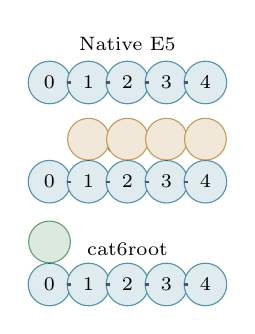
\begin{tikzpicture}[
    scale=0.9,
    every node/.style={font=\scriptsize},
    spine/.style={circle, draw=lumoCyan!80, fill=lumoCyan!15, minimum size=5.3mm},
    branch/.style={circle, draw=lumoAmber!80, fill=lumoAmber!18, minimum size=5.3mm},
    rootbranch/.style={circle, draw=lumoGreen!80, fill=lumoGreen!18, minimum size=5.3mm},
    edge/.style={draw=lumoGray, thick}
]
\node at (1.1,1.9) {Native E5};
\foreach \x/\n in {0/0,0.55/1,1.1/2,1.65/3,2.2/4} {
  \node[spine] (e\n) at (\x,1.35) {\n};
}
\foreach \a/\b in {e0/e1,e1/e2,e2/e3,e3/e4} \draw[edge] (\a)--(\b);

\node at (1.1,0.45) {cat9};
\foreach \x/\n in {0/0,0.55/1,1.1/2,1.65/3,2.2/4} {
  \node[spine] (c\n) at (\x,-0.05) {\n};
}
\foreach \x/\n in {0.55/a,1.1/b,1.65/c,2.2/d} {
  \node[branch] (c\n) at (\x,0.55) {};
}
\foreach \a/\b in {c0/c1,c1/c2,c2/c3,c3/c4,c1/ca,c2/cb,c3/cc,c4/cd} \draw[edge] (\a)--(\b);

\node at (1.1,-1.0) {cat6root};
\foreach \x/\n in {0/0,0.55/1,1.1/2,1.65/3,2.2/4} {
  \node[spine] (r\n) at (\x,-1.5) {\n};
}
\node[rootbranch] (rr) at (0,-0.9) {};
\foreach \a/\b in {r0/r1,r1/r2,r2/r3,r3/r4,r0/rr} \draw[edge] (\a)--(\b);
\end{tikzpicture}
\caption{The evaluated shapes. cat9 adds runner-up leaves to the depth-5 spine; cat6root keeps the spine and adds only a root sibling, reducing verifier work while preserving most of the acceptance gain.}
\label{fig:shapes}
\end{figure}

\section{GDN Scan and Replay Kernel}

The GDN recurrence is a stateful linear-attention update. For one value tile, the served kernel implements the same rank-1 update body used by the native path:
\begin{align}
S'_t &= \exp(g_t) S_{t-1}, \\
\Delta_t &= \beta_t \left(v_t - S'_t k_t\right), \\
S_t &= S'_t + \Delta_t k_t^\top, \\
o_t &= S_t q_t.
\end{align}
For a tree node \(i\), the invariant is \(S_i = \mathrm{native\_scan}(\mathrm{tokens}(\mathrm{root}\rightarrow i))\). This is simple to state and easy to violate in a packed GPU implementation \cite{yang2024gated}. A linearized tree scan is wrong whenever a branch follows a sibling in memory. If branch node \(b_1\) is a child of root \(n_0\), the required state is \(S_{b_1}=F(S_{n_0},x_{b_1})\), not \(F(S_{n_1},x_{b_1})\) for the previous packed spine node \(n_1\).

\begin{figure}[t]
\centering
\resizebox{\columnwidth}{!}{%
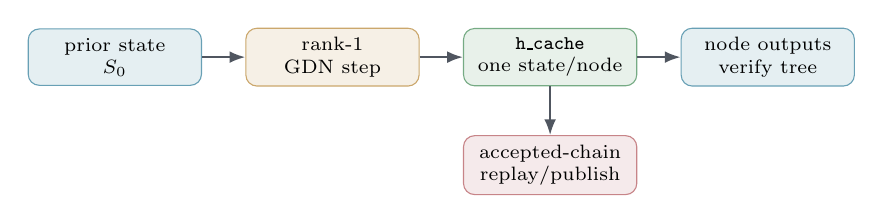
\begin{tikzpicture}[
    node distance=0.7cm,
    boxC/.style={rectangle, rounded corners, draw=lumoCyan!70, fill=lumoCyan!12, minimum width=2.2cm, minimum height=0.65cm, align=center, font=\scriptsize},
    boxA/.style={rectangle, rounded corners, draw=lumoAmber!70, fill=lumoAmber!12, minimum width=2.2cm, minimum height=0.65cm, align=center, font=\scriptsize},
    boxG/.style={rectangle, rounded corners, draw=lumoGreen!70, fill=lumoGreen!12, minimum width=2.2cm, minimum height=0.65cm, align=center, font=\scriptsize},
    boxR/.style={rectangle, rounded corners, draw=lumoRose!70, fill=lumoRose!12, minimum width=2.2cm, minimum height=0.65cm, align=center, font=\scriptsize},
    arrow/.style={-{Latex[length=2mm]}, thick, draw=lumoGray}
]
\node[boxC] (h0) {prior state\\\(S_0\)};
\node[boxA, right=0.55cm of h0] (step) {rank-1\\GDN step};
\node[boxG, right=0.55cm of step] (cache) {\code{h\_cache}\\one state/node};
\node[boxC, right=0.55cm of cache] (out) {node outputs\\verify tree};
\node[boxR, below=0.62cm of cache] (replay) {accepted-chain\\replay/publish};
\draw[arrow] (h0) -- (step);
\draw[arrow] (step) -- (cache);
\draw[arrow] (cache) -- (out);
\draw[arrow] (cache) -- (replay);
\end{tikzpicture}
}%
\caption{The scan verifies all candidate nodes with parent-indexed recurrent state. Replay re-executes only the accepted chain and publishes durable GDN/conv state.}
\label{fig:gdn}
\end{figure}

\begin{algorithm}[t]
\caption{Branch-local GDN scan and publication}
\label{alg:gdn}
\scriptsize
\begin{algorithmic}[1]
\REQUIRE Prior durable state \(S_0\), tree parent array \(p\), node features \(x_i\), accepted path \(A\)
\FOR{node \(i\) in topological tree order}
    \IF{\(p_i\) is root}
        \STATE \(S_{\mathrm{parent}} \leftarrow S_0\)
    \ELSE
        \STATE \(S_{\mathrm{parent}} \leftarrow \code{h\_cache}[p_i]\)
    \ENDIF
    \STATE \((o_i,S_i) \leftarrow \mathrm{GDNNodeStep}(S_{\mathrm{parent}},x_i)\)
    \STATE \(\code{h\_cache}[i] \leftarrow S_i\)
\ENDFOR
\STATE Device committer selects accepted node sequence \(A\)
\STATE \(S \leftarrow S_0\)
\FOR{node \(i\) in \(A\) in native order}
    \STATE \((o,S) \leftarrow \mathrm{GDNNodeStep}(S,x_i)\)
\ENDFOR
\STATE Publish only replayed \(S\) and the matching convolution state
\end{algorithmic}
\end{algorithm}

The kernel keeps a post-state for each padded node in \code{h\_cache}. That table has shape \([N_{\mathrm{PAD}}, BV, DIM_K]\) in fp32, where \(BV\) is the value-channel tile width. This is the main local resource constraint and the reason the kernel has an explicit tree-size boundary rather than an unbounded tree descriptor.

\subsection{BV, \(N_{\mathrm{PAD}}\), and Spill Boundary}

We write \code{BV16/w8} for a value tile of 16 rows launched with eight Triton warps. The shipped scan locks \code{BV=16} and \code{num\_warps=8}; the native packed-decode geometry audited from the pinned runtime is \(BV=32\), one warp, and three stages. \(N_{\mathrm{PAD}}\) is the next power-of-two span used by the static tree masks and unrolled Triton loops. Thus a six-node cat6root tree occupies pad8, while nine-node cat9 and deeper deployed families occupy pad16; the runtime fails loud for activation rings with \code{n\_pad} greater than 16 \cite{lumo2026artifact}.

The resource model is simple enough to expose. With \(DIM_K=128\), the scan's cached post-state footprint is
\begin{equation}
M_h = N_{\mathrm{PAD}}\cdot BV\cdot DIM_K\cdot4\;\mathrm{bytes}.
\end{equation}
The corresponding register-pressure estimate for the cache alone is
\begin{equation}
R_h \approx \frac{N_{\mathrm{PAD}}\cdot BV\cdot DIM_K}{32W},
\end{equation}
where \(W\) is the warp count. This estimate is not a substitute for ptxas, because the working tile and live q/k/v/g/beta values add pressure, but it predicts the failure mode: the full tree cache grows with padded node count, not with batch size.

\begin{table}[t]
\caption{GDN scan geometry and the pad16 resource boundary.}
\label{tab:bv-npad}
\centering
\scriptsize
\begin{adjustbox}{width=\columnwidth}
\begin{tabular}{L{0.27\columnwidth} C{0.15\columnwidth} L{0.25\columnwidth} L{0.25\columnwidth}}
\toprule
Geometry & \code{h\_cache} & Resource fact & Role \\
\midrule
Native one-node shape \(BV32/w1/s3, N=1\) & 16 KB & No full-tree state table. & Native packed-decode reference shape. \\
\rowsep
Full-tree native shape \(BV32/w1/s3, N=16\) & 256 KB & About 2048 cache fp32 values/lane before other live values; catastrophic spill. & Not deployable as a cached tree scan. \\
\rowsep
Deployed cat9 scan \(BV16/w8, N=16\) & 128 KB & Measured 254 regs/thread and 0 spill. & Shipped deepest tree-scan geometry. \\
\rowsep
cat6root scan \(BV16/w8, N=8\) & 64 KB & Half the cached state of cat9. & Explains near-native verify time with root-sibling gain. \\
\rowsep
Future pad32 \(BV16/w8, N=32\) & 256 KB & Register/SRAM hard wall for the cached scan. & Requires recompute or replay-style ancestry. \\
\bottomrule
\end{tabular}
\end{adjustbox}
\end{table}

This is why \(BV\) is not a free equivalence dial. Shrinking to \(BV=4\) reduces the cache, but it changes the tensor shape from native's \([32,128]\) reduction to \([4,128]\), changes compiler layout and reduction order, and increases the number of value-tile programs. The deployed \(BV16/w8\) point is not chosen because it proves native SASS identity; it is chosen because it is output-bit-exact to the banked scan reference at \(N_{\mathrm{PAD}}=1\) and \(16\), has measured zero spill, and preserves enough tile width for speed. The remaining bit-exactness obligation is against the native packed-decode geometry, which is why the code keeps an explicit diagnostic override and a separate recompute-from-spine route.

The spill boundary applies to the scan, not to publication. The accepted-path replay kernel carries one \([BV,DIM_K]\) state tile and re-executes only the committed chain, so its state footprint is \(O(1)\) in tree size. The recompute-from-spine scan variant uses the same idea for verification: recompute each node's ancestry from the spine instead of caching every node post-state. That route can launch at native \(BV32/w1/s3\), removes the pad16 state-cache wall, and is the right path for trees wider than the current deployed family. Its cost is extra rank-1 replay work, not local-memory spill on the saturated decode bandwidth path.

The scan and replay call the same node-step body. This is the key guard against a verifier that accepts under one recurrence but publishes under another. The body applies the native gate convention, beta's bf16 round trip, q/k normalization by division rather than reciprocal-square-root, output scaling, the rank-1 state update, and the carried-state bf16 boundary after output computation. These numeric seams are not cosmetic. In speculative decoding, a small branch-local numerical difference matters if it changes a clear-margin argmax or a residual sampling decision after many recurrent and attention layers.

The publication path also handles non-attention state. After the device committer chooses a path, the runtime remaps GDN state and convolution state using the accepted node rows, with gather-before-scatter ordering so overlapping source and destination columns cannot race. The convolution prior for the next event is taken from the accepted leaf before remap. This makes the durable state exactly the replayed native-order chain, while rejected rows remain temporary verifier state in \code{h\_cache}.

\section{Experimental Setup}

The target checkpoint is the public Hugging Face model \code{Qwen/Qwen3.6-27B-FP8}, a 64-layer hybrid model whose documented layout has 48 GDN recurrent layers and 16 softmax-attention layers \cite{qwen2026qwen36fp8}. The serving environment mounts it at \code{/models/qwen3.6-27b-fp8} and exposes it as \code{qwen3.6-27b} on GB10. The source-of-truth runtime is a \code{vllm/vllm-openai} image pinned to digest \texttt{sha256:3dbe092ec5b2cef63b6}\allowbreak\texttt{104d33fa75d6ce53a7870962}\allowbreak\texttt{529ada69f78bbbc38e776}, corresponding to vLLM 0.19.2rc1.dev134+gfe9c3d6c5, plus the forked FA2 \code{.so} swap and the boot-time tree-GDN patcher. The clean B=1 tree arms use the forked FA2 tree-server launcher; cat9 also has a locked wrapper, native E5 uses the native speed launcher, and the B=1 deploy wrapper pins \code{GPU\_UTIL=0.82}, \code{MAX\_NUM\_SEQS=1}, \code{MAX\_MODEL\_LEN=131072}, and \code{FR13\_DEVICE\_MULTIDRAFT=1}. The mounted model path and runtime image are pinned; the immutable Hugging Face snapshot hash inside the mount was not captured and is listed as a reproduction limitation. The workload is four SWE/Codex tasks in clean B=1 mode, temperature 0.6, with true sequential windows and \code{num\_running} near zero.

Speed and empirical-equivalence evidence are measured in separate modes. Speed runs disable heavy capture/oracle probes; equivalence runs enable recurrent-oracle capture and p-rescore. This separation is not bookkeeping. Several earlier readings were confounded by raw prompt probes, B=4 co-residency, instrumentation overhead, or denominator mistakes, so the final result reports token-weighted decode throughput, per-request latency, p-rescore equivalence, and end-to-end wall caveats as different measurements.

\subsection{Speed and Equivalence Infrastructure}

The final gate uses the deployment regime, not the earlier raw-prompt microbench regime. The raw \code{/v1/completions} probes were useful for kernel debugging, but they produced off-distribution \code{<think></think>} loops and cross-boot trajectory forks that made accept/event non-comparable. The final runs use the SWE/Codex agent loop through the deployment proxy and bracket vLLM metrics per task. Engagement is fail-loud: native E5 must show five draft tokens per draft event, a tree arm must show \(|T|\), and tree metadata must carry parent indices and accepted-path rows.

Speed mode is instrumentation-off except for low-overhead counters. It records raw vLLM deltas for decode seconds, draft events, accepted draft tokens, and generated tokens. When the pure-decode GPU timer is armed, \code{FR13\_SFWD\_GPU\_TIMER} records asynchronous CUDA events around model forward only on uniform decode steps; it excludes prefill and mixed prefill+decode steps and drains completed events without per-step synchronization. Optional \code{FR13\_DFWD\_GPU\_TIMER} and \code{FR13\_CFWD\_GPU\_TIMER} sidecars attribute drafter and committer spans, but these attribution timers are not substitutes for the deployment-speed gate.

Equivalence mode is instrumentation-on and intentionally not used for speed. The proxy pair-dump is converted back to a served-token source stream, and \code{fr13\_recurrent\_decode\_oracle.py} rescoring runs each arm's own no-spec recurrent decode path with speculative configuration disabled. This corrected an earlier oracle-frame mistake: chunked re-prefill is not the same as single-step recurrent decode for this hybrid target. The p-rescore then compares the served stream against the arm-local recurrent oracle and counts clear-margin argmax flips. That is why the paper reports a within-native-floor equivalence gate, not a bit-exact trace claim and not a speed number from an oracle-enabled boot.

\begin{table*}[t]
\caption{Clean B=1 decode result. Throughput delta is token-weighted decode TPS relative to native E5. Accept/event counts accepted draft tokens; committed tokens/event equals accept/event plus one guaranteed verifier token.}
\label{tab:results}
\centering
\scriptsize
\begin{adjustbox}{width=\textwidth}
\begin{tabular}{L{0.15\textwidth} L{0.24\textwidth} C{0.10\textwidth} C{0.12\textwidth} C{0.09\textwidth} C{0.09\textwidth} C{0.09\textwidth}}
\toprule
Arm & Tree & Per-request TPS & Token-weighted TPS & Delta & s/fwd\_gpu & Accept/event \\
\midrule
Native E5 & Native 5-step MTP spine & 17.80 & 18.80 & baseline & 0.137 & 3.11 \\
\rowsep
cat9 & 9-node caterpillar: 5-spine + 4 leaves & 18.44 & 22.63 & +20.4\% & 0.144 & 3.64 \\
\rowsep
cat6root & 6-node root branch: 5-spine + root sibling & 18.51 & 23.88 & +27.0\% & 0.138 & 3.82 \\
\bottomrule
\end{tabular}
\end{adjustbox}
\end{table*}

Table~\ref{tab:results} is the core speed result. The accept/event column counts accepted draft tokens only. Each verify event also commits the verifier's guaranteed next token, so committed tokens/event is accept/event plus one: native E5 moves from 3.11 accepted drafts/event to 4.11 committed tokens/event, and cat6root moves from 3.82 to 4.82. This is a 17.2\% committed-token gain while verify-forward time remains essentially native. The gain comes from the root sibling's position in the tree: it is a depth-0 alternative that recovers events native MTP loses when the first spine token is rejected, instead of spending most extra work on deeper leaves whose ancestors must all survive.

The three speed views are related but not interchangeable. Multiplying the committed-token gain by the pure verify-forward sidecar would predict a roughly 16--17\% forward-only improvement, because \(0.137/0.138\) s/fwd is nearly flat. The reported +27.0\% is instead token-weighted deploy TPS: total generated decode tokens divided by request decode seconds across the clean B=1 window. That denominator includes non-forward decode overhead and the weighting concentrates on long turns where most tokens are produced. The per-request-equal view gives +4.0\% because it weights a short shell-tool call like a long edit turn. This paper reports all three numbers so the +27.0\% headline is not read as a forward-only algebra or an end-to-end task-wall claim.

The request anatomy explains why these metrics differ. In the cat6root B=1 trace, 24.7\% of turns have at most 64 output tokens, but those turns account for only 3\% of output tokens; they are mostly short shell-tool calls in the Codex agent loop. Speculative decoding helps more on longer turns, so per-request-equal averaging undercounts the decode-token gain. This does not imply a 27\% end-to-end task-wall gain, because the same workload repeatedly sends roughly 11k--14k prompt tokens and prefix caching is off for this hybrid setup. The final B=1 receipts do not promote a clean task-wall speedup; they establish that task wall improves by less than the decode-only gain unless deployment work reduces repeated prefill or overlaps streams.

\section{Empirical Equivalence Evidence and Measurement Discipline}
\label{sec:lossless}

The empirical equivalence claim in this artifact is closure within the observed native recurrent-oracle flip floor. The exact B=1 depth-5 p-rescore compares each arm against its own no-spec recurrent oracle under temperature 0.6. Native E5 has 630 clear-margin flips over 4,883 positions, or 12.90\%; cat9 has 645 over 4,858, or 13.28\%; cat6root has about 636 over about 4,860, or 13.09\%. Both tree arms are within the native E5 floor by less than one position-level standard error, but this is not a TV-distance estimate and not a request-cluster bootstrap.

\begin{table}[t]
\caption{Empirical equivalence closure gates and interpretation.}
\label{tab:lossless}
\centering
\scriptsize
\begin{adjustbox}{width=\columnwidth}
\begin{tabular}{L{0.27\columnwidth} L{0.35\columnwidth} L{0.28\columnwidth}}
\toprule
Gate & Checked & Status \\
\midrule
Depth-5 p-rescore & E5/cat9/cat6root temp-0.6 recurrent oracle. & Within native floor. \\
\rowsep
GDN scan A/B & \(BV16=BV32=0.0\) in controlled scan. & Scan alone is clean. \\
\rowsep
Native path oracle & Path-local state versus native decode order. & Core invariant. \\
\rowsep
Device committer & Same residual-mix rule on device. & Residual-rule gate. \\
\rowsep
Broad cat9 floor & Big-denom deployment consolidation. & Overlapping floor intervals. \\
\bottomrule
\end{tabular}
\end{adjustbox}
\end{table}

The statistical caveat matters. The p-rescore sample has roughly 4.9k positions per arm, but positions inside one SWE/Codex turn are correlated. The result is therefore clean B=1 closure for the observed sample, not a universal guarantee across all seeds, batch sizes, or prompt distributions. Request-cluster bootstrap, additional seeds, and full distribution-distance measurements are follow-up gates.

The measurement infrastructure is part of the contribution because it prevented false wins and false losses. The canonical formulas are:
\begin{align}
\mathrm{s/fwd\_gpu} &= \frac{\mathrm{decode\ forward\ GPU\ seconds}}{\mathrm{pure\ decode\ drafts}}, \\
\mathrm{accept/event} &= \frac{\mathrm{accepted\ draft\ tokens}}{\mathrm{draft\ events}}, \\
\mathrm{committed/event} &= \mathrm{accept/event}+1, \\
\mathrm{deploy\ TPS} &= \frac{\mathrm{request\ decode\ tokens}}{\mathrm{request\ decode\ seconds}}.
\end{align}
Probe separation, deployment-path-only measurement, token weighting, and oracle-mode separation are all needed to make the numbers interpretable. This is why raw \code{/v1/completions} probes, B=4 screens, and oracle-enabled equivalence traces are not treated as substitutes for the clean B=1 deployment-speed gate.

\section{Design Evolution and Negative Results}

The failure library explains why the final verifier has its particular contract. It separates three questions that can otherwise blur together: whether the verifier preserves the target distribution within the native floor, whether the kernel is fast enough to matter, and whether the measurement regime is timing the served path. Table~\ref{tab:negative} condenses the HTML failure library into paper form.

\begin{table*}[t]
\caption{Negative results and superseded interpretations that shaped the final verifier. These are not all mathematical impossibilities; several are rejected only as served-proof routes for this artifact.}
\label{tab:negative}
\centering
\scriptsize
\begin{adjustbox}{width=\textwidth}
\begin{tabular}{L{0.18\textwidth} L{0.25\textwidth} L{0.28\textwidth} L{0.19\textwidth}}
\toprule
Route or interpretation & Why it looked plausible & What failed & Paper consequence \\
\midrule
Attention-mask-only tree & Tree verification for attention-only LLMs mainly needs ancestry. & GDN rows still carried sibling-contaminated recurrent state. & Attention ancestry is necessary but not sufficient. \\
\rowsep
Shared packed recurrent accumulator & Co-resident rows are efficient if packed sequentially. & Packed order is not native branch order, so sibling states leak. & The scan must be parent-indexed and branch-local. \\
\rowsep
STree-style state sharing as direct transplant & STree gives the right stateful-tree problem lens. & Algebraic state construction is not the same as matching served bf16/fp8 GDN writeback. & STree is prior work, not the served-realization proof. \\
\rowsep
Triton \code{TREE\_ATTN} as proof path & It can express a tree mask. & It is not the same FA2 decode realization as native serving. & The reported path uses a forked FA2 tree-bias decode kernel. \\
\rowsep
WY / whole-tree algebra & It could reduce state traffic and expose more parallelism. & Different summation trees and bf16 boundaries are not the native sequential verify oracle. & Kept as future speed work; not the equivalence proof route. \\
\rowsep
Literal \(0.0\) max-abs as only equivalence bar & Bit equality is easy to state. & Native recurrent-oracle comparisons already have a numerical flip floor. & The paper uses within-native-floor p-rescore, not bit-exact intermediate equality. \\
\rowsep
cat10 and broad B=4 screens & Wider trees and batching are deployment-relevant. & Contaminated reads violated the expectation that a strict tree superset should not accept fewer spine tokens than native. & Clean B=1 is the mechanism proof; B=4 needs a refreshed carrier-clean run. \\
\rowsep
Per-request TPS as headline & It is a latency-friendly summary. & It weights a short shell-tool turn like a long edit turn. & Token-weighted decode TPS is the throughput headline; per-request TPS is a caveat. \\
\bottomrule
\end{tabular}
\end{adjustbox}
\end{table*}

Several rows are useful future work rather than dead ends. WY-style whole-tree algebra may still become a speed route if it can be tied back to the served sequential oracle. Cache-side or radix-style state sharing in vLLM would also be complementary to the current verifier rather than a replacement for it. The important point is that none of those routes is allowed to stand in for accepted-chain replay, path-local GDN state, or the deployment/equivalence separation used in the reported result.

\section{Threats to Validity}

The result is strong for clean B=1 decode throughput and within-floor closure under the current recurrent-oracle p-rescore. It does not claim that every deployment bottleneck is solved.

\begin{itemize}[leftmargin=*,noitemsep]
    \item \textbf{Equivalence sample size.} The exact cat9/cat6root p-rescore is a 40-turn B=1 sample per arm. The position-level standard error is informative but optimistic because positions within a turn are correlated; request-level bootstrap and more seeds remain open.
    \item \textbf{Decode is not full task wall.} The +27.0\% number is decode throughput. SWE/Codex requests repeatedly send large repository context, and prefix caching is off for this hybrid setup, so end-to-end wall gains are smaller; the final receipts do not contain a clean promoted task-wall number.
    \item \textbf{B=4 needs refreshed treatment.} The clean mechanism result is B=1. Batching changes co-residency, scheduler pressure, and prefill/decode overlap, so the old B=4 diagnostics are not a final verdict.
    \item \textbf{Stage D timing is open.} Drafter, verify forward, and isolated committer compute are near E5, but live phase attribution still needs direct step-wall timers.
    \item \textbf{Model snapshot packaging.} The model name and local mount are pinned, but the immutable Hugging Face snapshot hash inside the mount was not captured in the current receipts.
\end{itemize}

\section{Canonical Configuration}

The shipped cat9 and cat6root arms share one tree-serving configuration. The only intended per-arm difference is the speculative tree shape: cat9 is a 9-node depth-5 spine plus leaves, while cat6root is a 6-node depth-5 spine plus root sibling. Table~\ref{tab:config} lists the load-bearing choices most likely to invalidate the result if changed.

\begin{table}[t]
\caption{Load-bearing configuration choices in the shipped tree path.}
\label{tab:config}
\centering
\scriptsize
\begin{adjustbox}{width=\columnwidth}
\begin{tabular}{L{0.33\columnwidth} L{0.57\columnwidth}}
\toprule
Surface & Choice \\
\midrule
Tree mode & \code{FR10\_ENABLE\_TREE\_GDN=1}, \code{FR10\_DECODE\_MODE\_DEFAULT=tree\_mtp}. \\
\rowsep
Attention & \code{FR13\_FA2\_TREE\_BIAS=1}, \code{FR13\_FA2\_PREFILL\_NATIVE=1}. \\
\rowsep
GDN scan geometry & \code{BV=16}, \code{num\_warps=8}, activation-ring \code{n\_pad}\(\leq16\); cat6root uses pad8 and cat9 uses pad16. \\
\rowsep
GDN batch variance fix & \code{LUMO\_FB\_KERNEL\_ROWS=1}, \code{LUMO\_FB\_PROJ\_PAD\_ROWS=16}. \\
\rowsep
Committer & \code{FR13\_DEVICE\_MULTIDRAFT=1} default-on for tree arms. \\
\rowsep
Safety & \code{FR10\_ALLOW\_LINEAR\_FALLBACK} unset. \\
\rowsep
Operational B=1 & \code{GPU\_UTIL=0.82}, \code{MAX\_NUM\_SEQS=1}. \\
\bottomrule
\end{tabular}
\end{adjustbox}
\end{table}

The committer row follows the later bake addendum: the older canonical-config catalog still lists \code{FR13\_DEVICE\_MULTIDRAFT} as diagnostic/off, while the addendum records that it was baked default-on for tree arms after verifying that native E5 does not read the tree committer gate. Some flags remain explicit on purpose. The FA2 tree-bias and native-prefill flags are default-off in the patcher to preserve patch idempotency anchors; baking them would require a separate re-patch verification task. The fixed-row in-projection pad should not be baked globally because it can perturb native E5 bytes, which define the recurrent-oracle baseline.

\section{Conclusion}

\sys{} turns a token tree into a served verifier for a recurrent hybrid language model by treating recurrent state as part of the tree contract. Attention ancestry is necessary, but not sufficient. The shipped path adds FA2 tree bias for softmax layers, branch-local GDN scan/replay for recurrent layers, and accepted-chain-only state publication for vLLM. Under the clean B=1 deployment gate, cat6root improves token-weighted decode throughput by 27.0\% while closing within the observed native recurrent-oracle flip floor. The result should be read with its caveats attached: decode-only, B=1, 40-turn p-rescore, no request-cluster bootstrap, no full distribution-distance estimate, prefill-heavy workload, and open B=4/Stage D follow-up.

\section*{Artifact and Source Trail}

The source blueprint is the live GitHub Pages paper, fetched and byte-matched to the local \code{gh-pages} worktree on June 18, 2026 \cite{lumo2026artifact}. This provenance is intentionally separated from the main technical framing. The consolidated source receipts are the deployed TPS correction, B=1 equivalence verdict, request anatomy, Stage D localization, vLLM source-of-truth ledger, launchers, FA2 fork correction, GDN tree kernel, vLLM tree wiring patch, device multidraft committer, measurement harness, canonical config ledger, and bake addendum \cite{lumo2026receipts}.

\label{ReferencesStart}
\bibliographystyle{ieeetr}
\bibliography{ref}

\end{document}
